\documentclass[aspectratio=169, 11pt]{beamer}

% ==================== ВЫБОР ЯЗЫКА И КОДИРОВКИ ====================
\usepackage[utf8]{inputenc}
\usepackage[russian]{babel} % Если нужен английский, замените на \usepackage[english]{babel}
\usepackage{amsmath, amsfonts, amssymb, pifont} % Для формул
\usepackage{graphicx} % Для вставки картинок
\usepackage{booktabs} % Для красивых таблиц
\usepackage{csquotes} % Для умных кавычек
\usepackage{hyperref}

% ==================== НАСТРОЙКА ТЕМЫ И ЦВЕТОВ ====================
% Используем тему Madrid как основу (она дает полосу вверху)
\usetheme{Madrid}
% Переопределяем цвета для более современного вида (синий + бирюзовый)
\definecolor{myblue}{RGB}{0, 80, 158}   % Темно-синий
\definecolor{myteal}{RGB}{0, 150, 180}  % Бирюзовый для акцентов

% Устанавливаем цвета элементов
\setbeamercolor{palette primary}{bg=myblue, fg=white}
\setbeamercolor{palette secondary}{bg=myteal, fg=white}
\setbeamercolor{palette tertiary}{bg=myblue!80!black, fg=white}
\setbeamercolor{structure}{fg=myblue} % Цвет маркеров и ссылок
\setbeamercolor{titlelike}{parent=palette primary} % Цвет заголовков

% Убираем навигационные иконки (делает слайды чище)
\setbeamertemplate{navigation symbols}{}

% Делаем точки в оглавлении более круглыми
\setbeamertemplate{section in toc}{\inserttocsectionnumber.~\inserttocsection}

% ==================== НАСТРОЙКА КОЛОНТИТУЛОВ ====================
% Добавляем номер слайда в нижний колонтитул
\setbeamertemplate{footline}{
	\leavevmode%
	\hbox{%
		\begin{beamercolorbox}[wd=\paperwidth,ht=2.25ex,dp=1ex,center]{author in head/foot}%
			\usebeamerfont{author in head/foot}\insertshorttitle\hfill\insertframenumber{} / \inserttotalframenumber
	\end{beamercolorbox}}%
	\vskip0pt%
}



% ==================== ИНФОРМАЦИЯ О ДОКУМЕНТЕ ====================
\title[Комплексный подход к дедуктивной верификации реализаций умножения матриц]{Комплексный подход к дедуктивной верификации реализаций умножения матриц}
\subtitle{\scriptsize{По итогам участия в Летнем Системном Буткемпе от лаборатории YADRO, НГУ}}
\institute{\small{Семинар теоретического и экспериментального программирования им. В.А. Непомнящего}}
\date{\small{22 сентября 2026 г.}}


% ==================== НАЧАЛО ДОКУМЕНТА ====================
\begin{document}


% ==================== ТИТУЛЬНЫЙ СЛАЙД ====================
\begin{frame}[plain]
	\titlepage
\end{frame}


% ==================== ОСНОВНАЯ ЧАСТЬ ====================
\begin{frame}{На пути к minigemm}
    Верифицировано ранее:
    \begin{itemize}
        \item Версия 0. Наивная реализация.
        \item Версия 1. С переставленными внутренними циклами.
    \end{itemize}
    \vspace{0.5cm}
    Работа в рамках Летнего Буткемпа лаборатории YADRO:
    \begin{itemize}
        \item Версия 2. С ассемблерными вставками.
    \end{itemize}
    \vspace{0.5cm}
    В течение этого семестра (до конца 2026 года):
    \begin{itemize}
    	\item Версия 3. С микроядром.
    \end{itemize}
\end{frame}


\begin{frame}{Визуализация умножения матриц}
	\begin{center}
		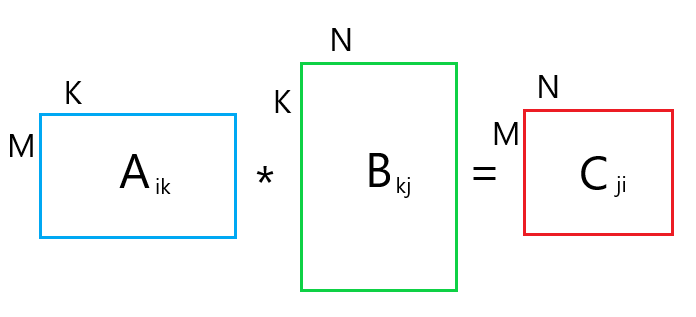
\includegraphics[scale=0.8]{img/matrix_mult.png}
	\end{center}
\end{frame}


\begin{frame}{Версия 0. Наивная реализация}
	\begin{center}
		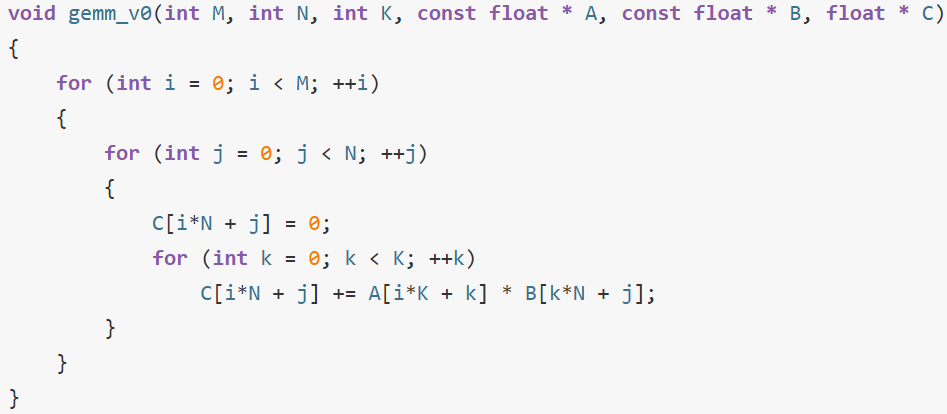
\includegraphics[scale=0.6]{img/gemm_v0.png}
	\end{center}
\end{frame}


\begin{frame}{Версия 1. С переставленными внутренними циклами}
	\begin{center}
		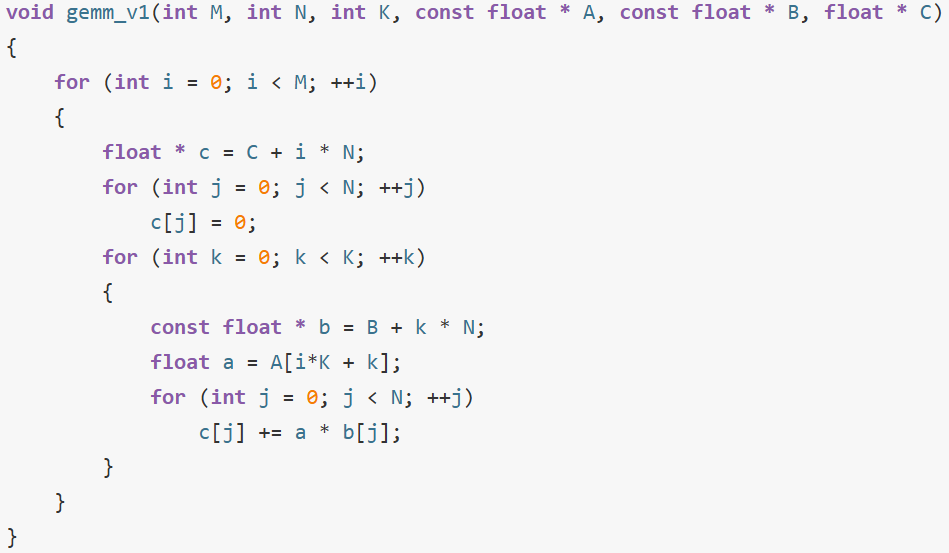
\includegraphics[scale=0.5]{img/gemm_v1.png}
	\end{center}
\end{frame}


\begin{frame}{Версия 2. С ассемблерными вставками}
	\begin{center}
		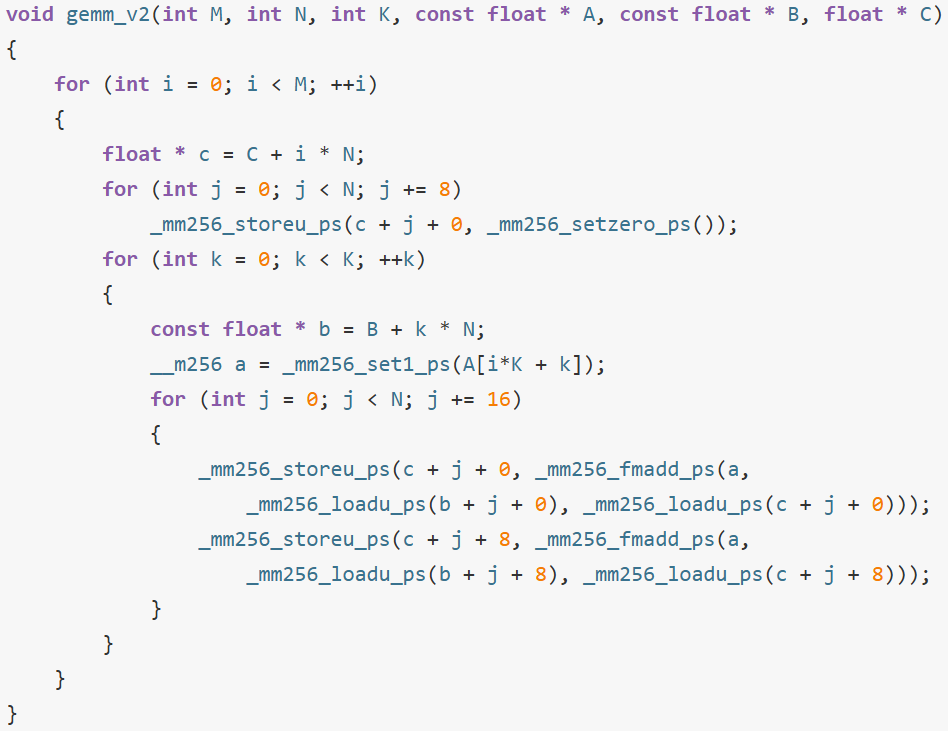
\includegraphics[scale=0.38]{img/gemm_v2.png}
	\end{center}
\end{frame}


\begin{frame}{Цели проекта}
	\begin{itemize}
		\item Цель 1. Выполнить реинжиниринг процесса дедуктивной верификации реализаций gemm\_v0, gemm\_v1
		\begin{block}{Мотивация}
			\begin{itemize}
				\item Повысить уровень автоматизации процесса верификации
				\item Заложить более надежную теоретическую и инженерную основу для верификации других алгоритмов умножения матриц
			\end{itemize}
		\end{block}
		
		\item Цель 2. Провести дедуктивную верификацию реализации gemm\_v2
		\begin{block}{Мотивация}
			\begin{itemize}
				\item Сделать ещё один шаг к верификации реализации алгоритма minigemm
			\end{itemize}
		\end{block}
	\end{itemize}
\end{frame}


\begin{frame}{Результаты для цели 1}
	\begin{enumerate}
		\item С учетом замечаний, сделанных в ходе изучения проделанной ранее работы, были проверены следующие гипотезы:
		\begin{enumerate}
			\item \ding{51} Удалить операцию означивания матрицы C нулями в наивном коде
			\item \ding{51} Удалить лишние separated в спецификациях
			\item \ding{55} По одному удалять valid\_read и valid в спецификациях
			\item \ding{55} Ослабить посылки в базе индукции индуктивных предикатов на n < 0 в теории предметной области
			\item \ding{55} По одному удалять assert в спецификациях
		\end{enumerate}
		\item Подготовлены отчетные материалы
	\end{enumerate}
\end{frame}


\begin{frame}{Результаты для цели 2}
	\begin{enumerate}
		\item Изучена предметная область
		\item Определены спецификации операций, входящих в ассемблерные вставки
		\item Расширена формальная теория предметной области на функции и предикаты из этих спецификаций
		\item Порождены условия корректности
		\item Доказаны условия корректности
		\item Подготовлены отчетные материалы
	\end{enumerate}

\end{frame}


\begin{frame}{Изучена предметная область}
    \begin{itemize}
        \item Основы дедуктивной верификации
        \item Основы машинного доказательства теорем
        \item Frama-C/WP + Why3
        \item SMT-решатели(Alt-Ergo, CVC4, CVC5, Z3, Vampire)
        \item Coq
        \item LLM для генерации скриптов доказательства
        \item Эвристики и стратегии доказательства
    \end{itemize}
\end{frame}


\begin{frame}{Определены спецификации операций, входящих в ассемблерные вставки}
    \begin{center}
        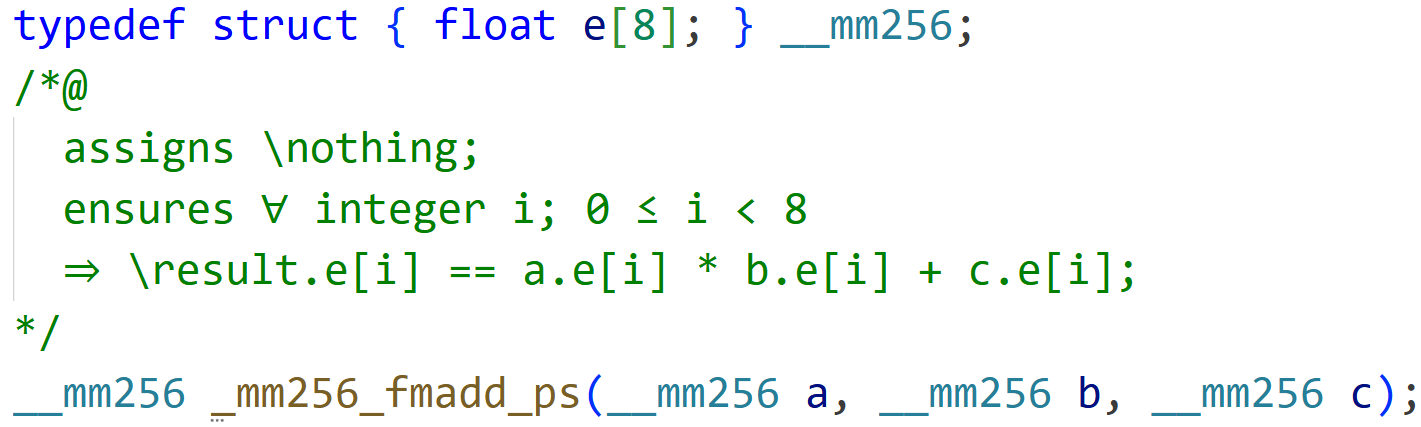
\includegraphics[scale=0.4]{img/typedef.png}
    \end{center}
\end{frame}


\begin{frame}{Расширена формальная теория предметной области на функции и предикаты из этих спецификаций}
    \begin{center}
        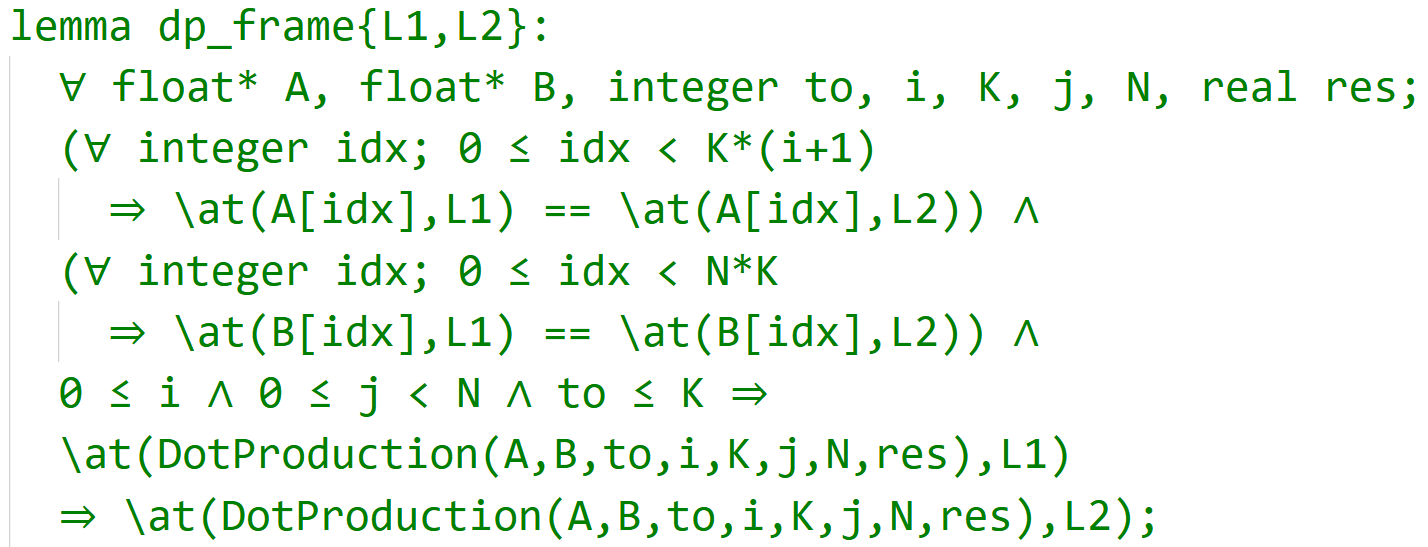
\includegraphics[scale=0.4]{img/dp_frame.png}
    \end{center}
\end{frame}


\begin{frame}{Порождены условия корректности}
	\begin{center}
		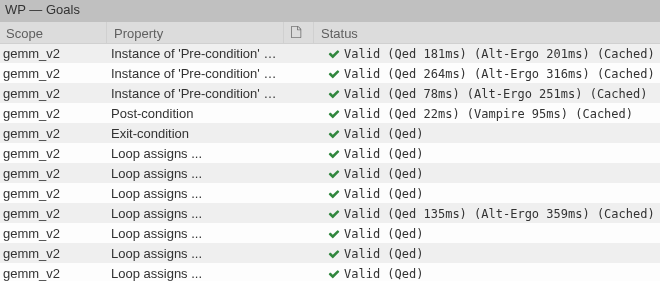
\includegraphics[scale=0.85]{img/goals.png}
	\end{center}
\end{frame}


\begin{frame}{Доказаны условия корректности}
	\begin{center}
    	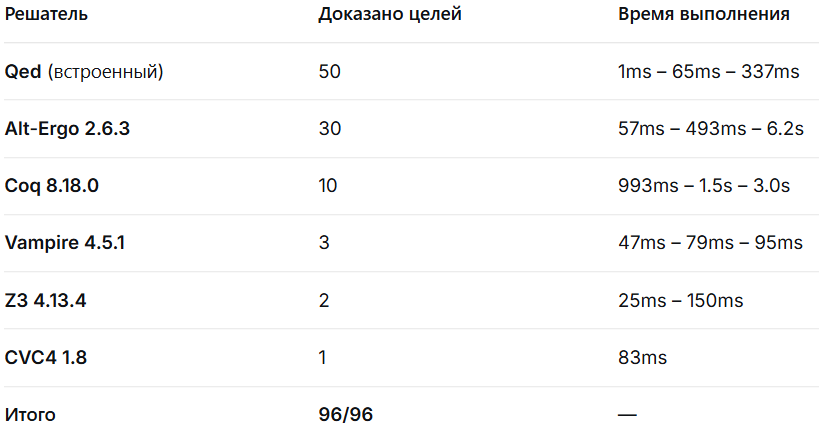
\includegraphics[scale=0.6]{img/output.png}
    \end{center}
\end{frame}


\begin{frame}{Подготовлены отчетные материалы}
    \begin{columns}[T]  % [T] - выравнивание по верхнему краю
        \begin{column}{0.6\textwidth}
            \begin{itemize}
                \item ReadMe с инструкцией по воспроизведению результатов
                \item Вики с описанием содержимого репозитория
                \item Файл с формальной спецификацией ассемблерных вставок
                \item Файл со аннотированной реализацией gemm\_v2
                \item Скрипты доказательств условий корректности в формате Coq
                \item Файл со спецификацией предметной области
                \item Файлы с модифицированными аннотированными реализациями gemm\_v0 и gemm\_v1
            \end{itemize}
        \end{column}
        \begin{column}{0.4\textwidth}
            \centering
            
\includegraphics[width=0.7\textwidth]{img/qr-code.png}\\
            \vspace{0.2cm}
            \small Репозиторий проекта: \url{https://github.com/ylab-nsu/sb26-trust-minigemm/}
        \end{column}
    \end{columns}
\end{frame}


\begin{frame}{Планы}
    \begin{itemize}
		\item Подготовка статьи по результатам проекта в рейтинговый журнал
		\item Верификация gemm\_v3
		\item ...
		\item Верификация minigemm
	\end{itemize}
\end{frame}


\begin{frame}{Команда проекта}
	\begin{figure}
	    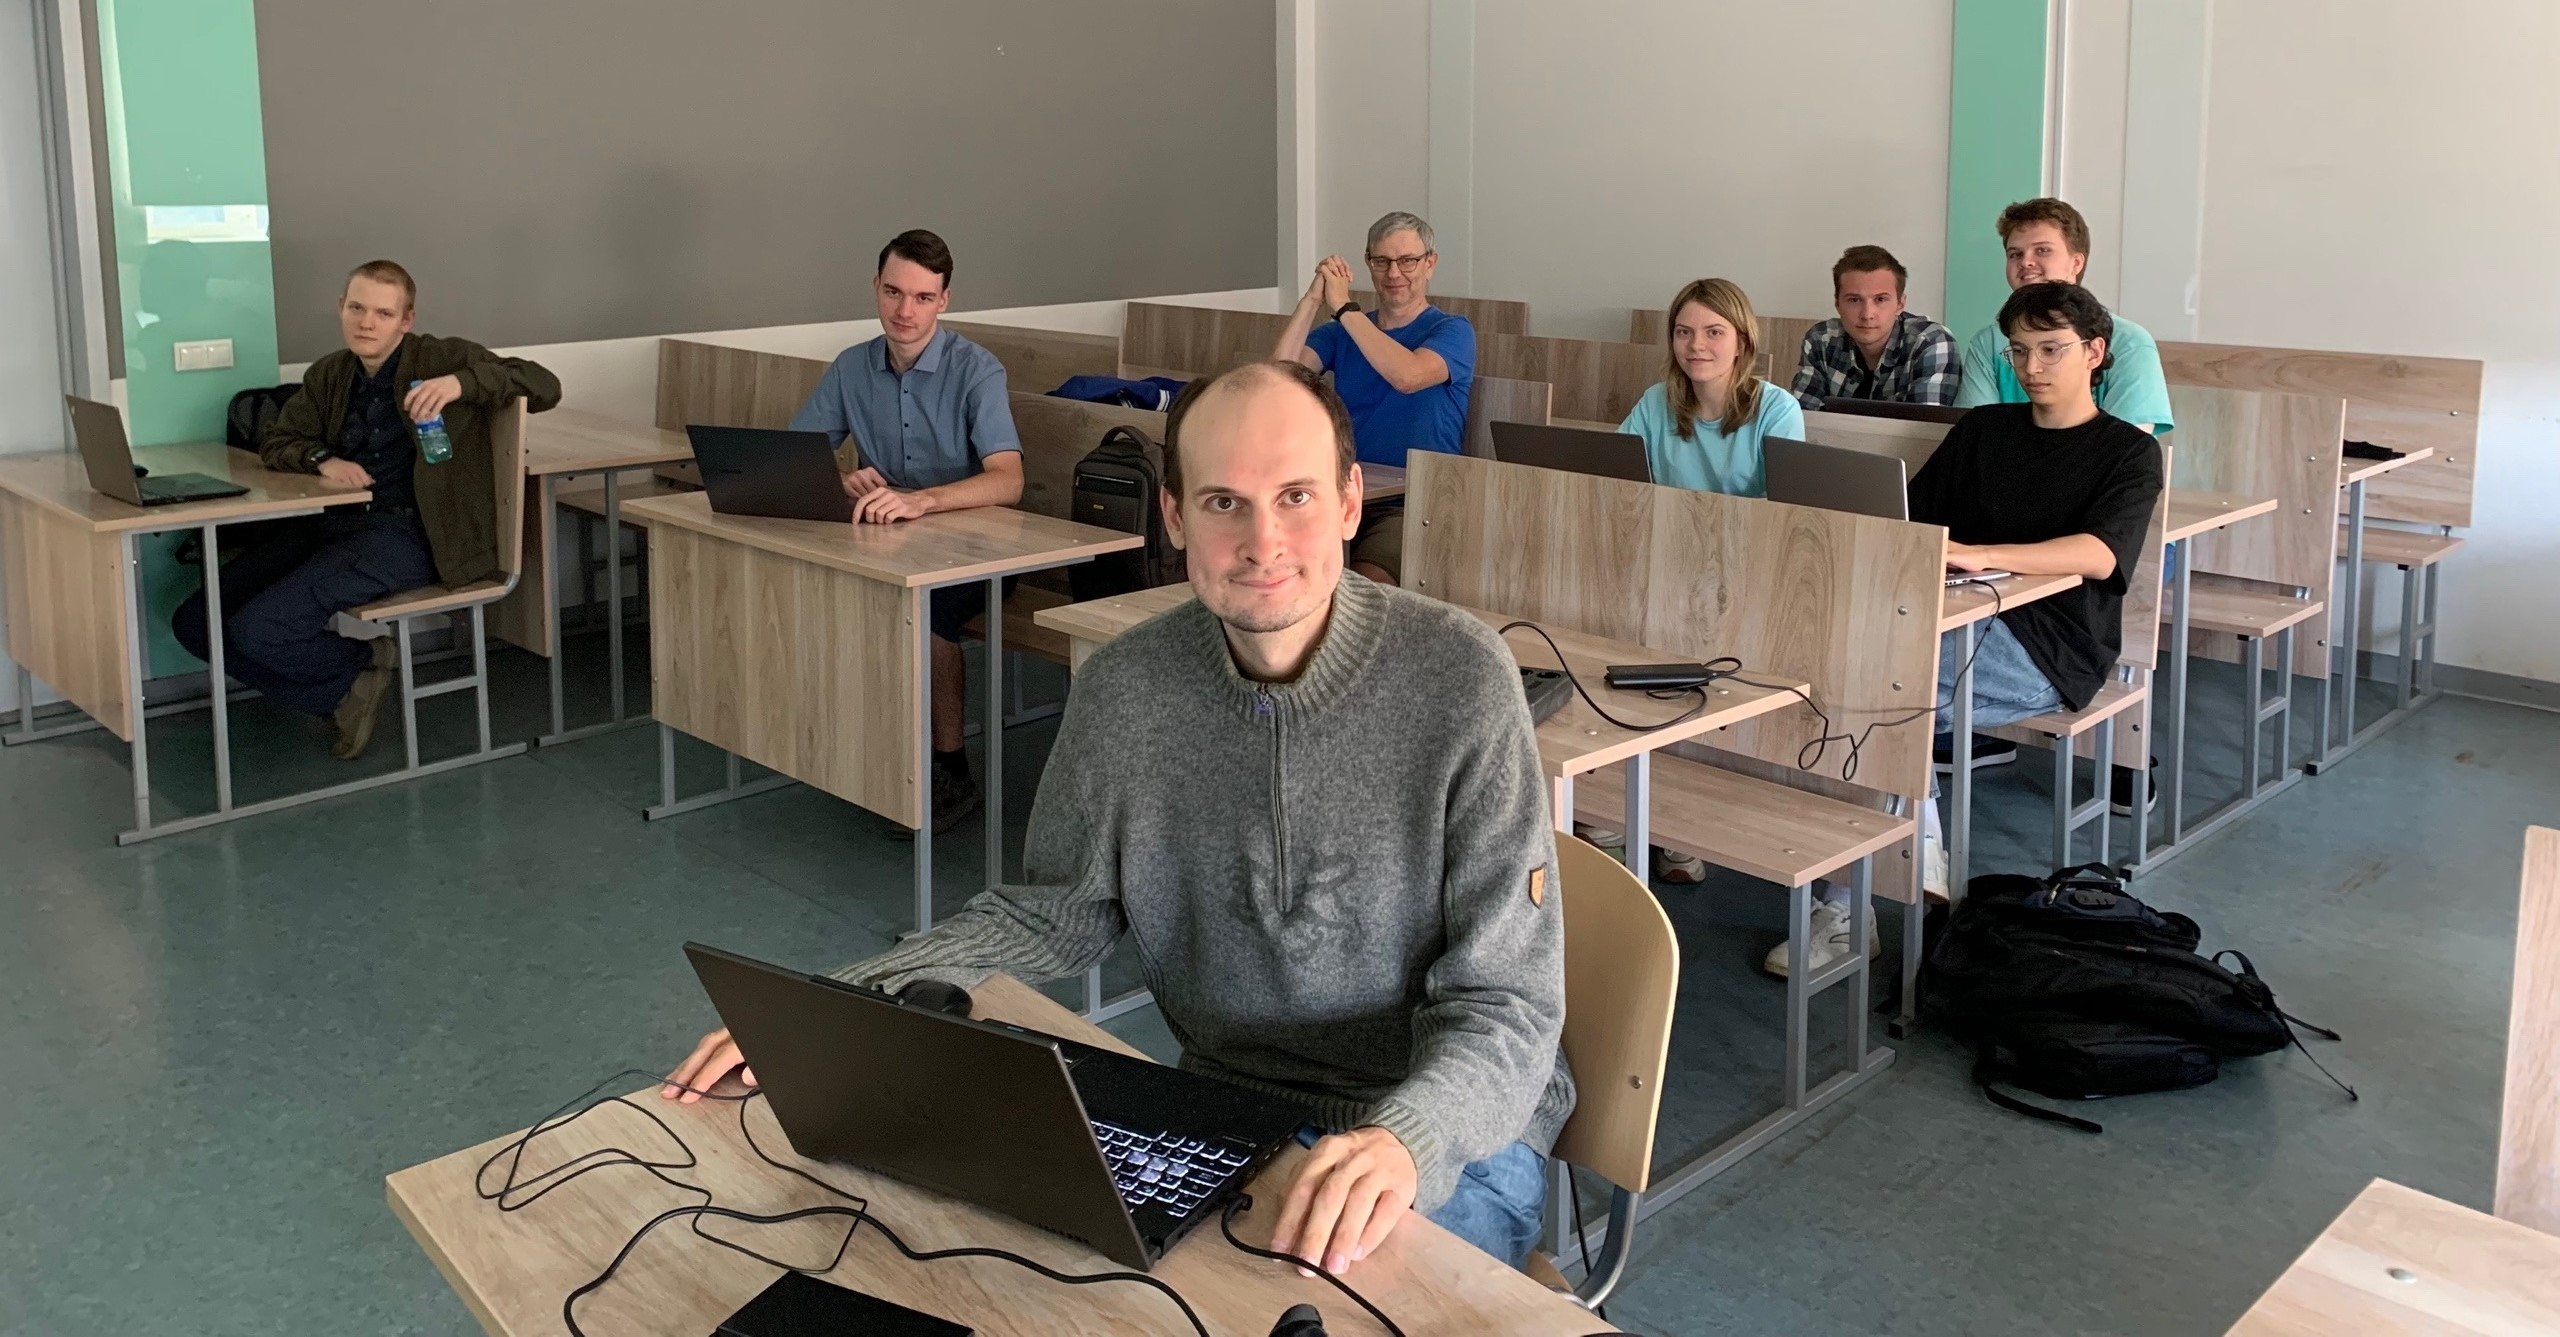
\includegraphics[scale=0.205]{img/team.jpg}
	\end{figure}
\end{frame}


\begin{frame}{Идея версии 3. С микроядром}
	\begin{center}
		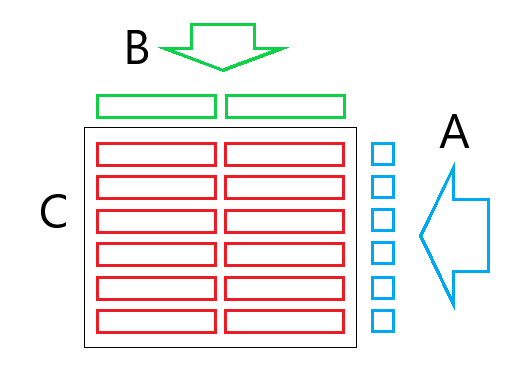
\includegraphics[scale=0.7]{img/micro_core.png}
	\end{center}
\end{frame}


\end{document}
